\begin{chapabstract}
\small{
This chapter introduces the experimental measurements of the performance of the Anomaly Detection technique presented in \autoref{c:Contribution-2}.
}\\
\begin{center}
\noindent\makebox[0.8\linewidth]{\rule{0.66\paperwidth}{0.4pt}}
\end{center}
\vspace{1cm}
\end{chapabstract}

\section{Experiment Setup}
\label{s:Experiment-Setup}
 The goal is to measure the performances of the A.D. technique against the Li\&Ma technique described in \autoref{ss:li-ma} to perform source detection. In particular, we are interested in applying the A.D. technique in the short-term and very short-term scenarios, in which the Li\&Ma analysis is not always applicable due to few photon counts. The integration times are set to 5 seconds and 1 second to simulate these settings. As stated in \autoref{s:contribution-2-use-cases}, the A.D. method is applied to two scientific use cases: serendipitous discoveries and observation triggered by a science-alerts. In the serendipitous discoveries settings, a GRB appears in the telescope's field of view; hence the totality of the event is observed. When the observatory reacts to a science alert, the telescopes will change their pointing to observe a sky region in which the GRB event is already started. The time taken to receive the science alert, change the pointing, and wait for enough data to perform the first analysis is variable: four values have been considered to model this delay: 15, 30, 60, and 120 seconds. 

As explained in \autoref{s:contribution-2-use-cases}, the sooner a detection is issued, the sooner other observatories can study the same source. Hence, the performances are measured regarding how fast the techniques are to issue $5\sigma$ detections and the number of those detections. The following section describes the test set generation process.
 
\subsection{Test set generation for performance evaluations}
\label{s:Experiment-Data}
The CTAO collaboration provides a Gamma-ray catalog providing almost 20 thousand GRB templates of known events [todo]. As stated in \autoref{c:Background}, Gamma-ray bursts are characterized by several key properties, including duration, prompt emission, and peak flux. The latter is a measure of the amount of energy that is emitted during the prompt gamma-ray emission. It is usually measured in units of $erg/s/cm^2$ and is one of the most important parameters for characterizing the luminosity of a GRB. GRBs can have a wide range of peak fluxes, from as low as $10^-9 erg/s/cm^2$ to as high as $10^-5 erg/s/cm^2$, depending on the distance and the intrinsic properties of the GRB. If the luminosity is too low, the GRB event will be indistinguishable from the background noise. Since the instrument response function that defines the background noise is fixed ($North\_z40\_5h\_LST$) there is no reason to simulate the entire GRB catalog since most of the GRBs will be impossible to detect. For these reasons, the mean of the background level has been considered a threshold to limit the number of simulations. In particular, a test set has been generated simulating all the templates whose peak flux is equal to greater to the background level mean minus $1\sigma$, to take into account the background fluctuations. Figure~\ref{f:exp-max-flux-distribution-E} shows the distribution of the peak flux of each GRB template and highlights the selected set. As explained in \autoref{dl3-simulator}, the simulation tool generates a photons list starting from a GRB template representing the GRB events seen by the telescopes as a list of photons whose energy and arrival direction is reconstructed. The simulation tool has been used to generate one simulated trial for each selected template. The resulting test set contains 419 trials with a peak flux in the interval $[2.6785e-10, \infty]$.
\begin{figure}[t]
\centering
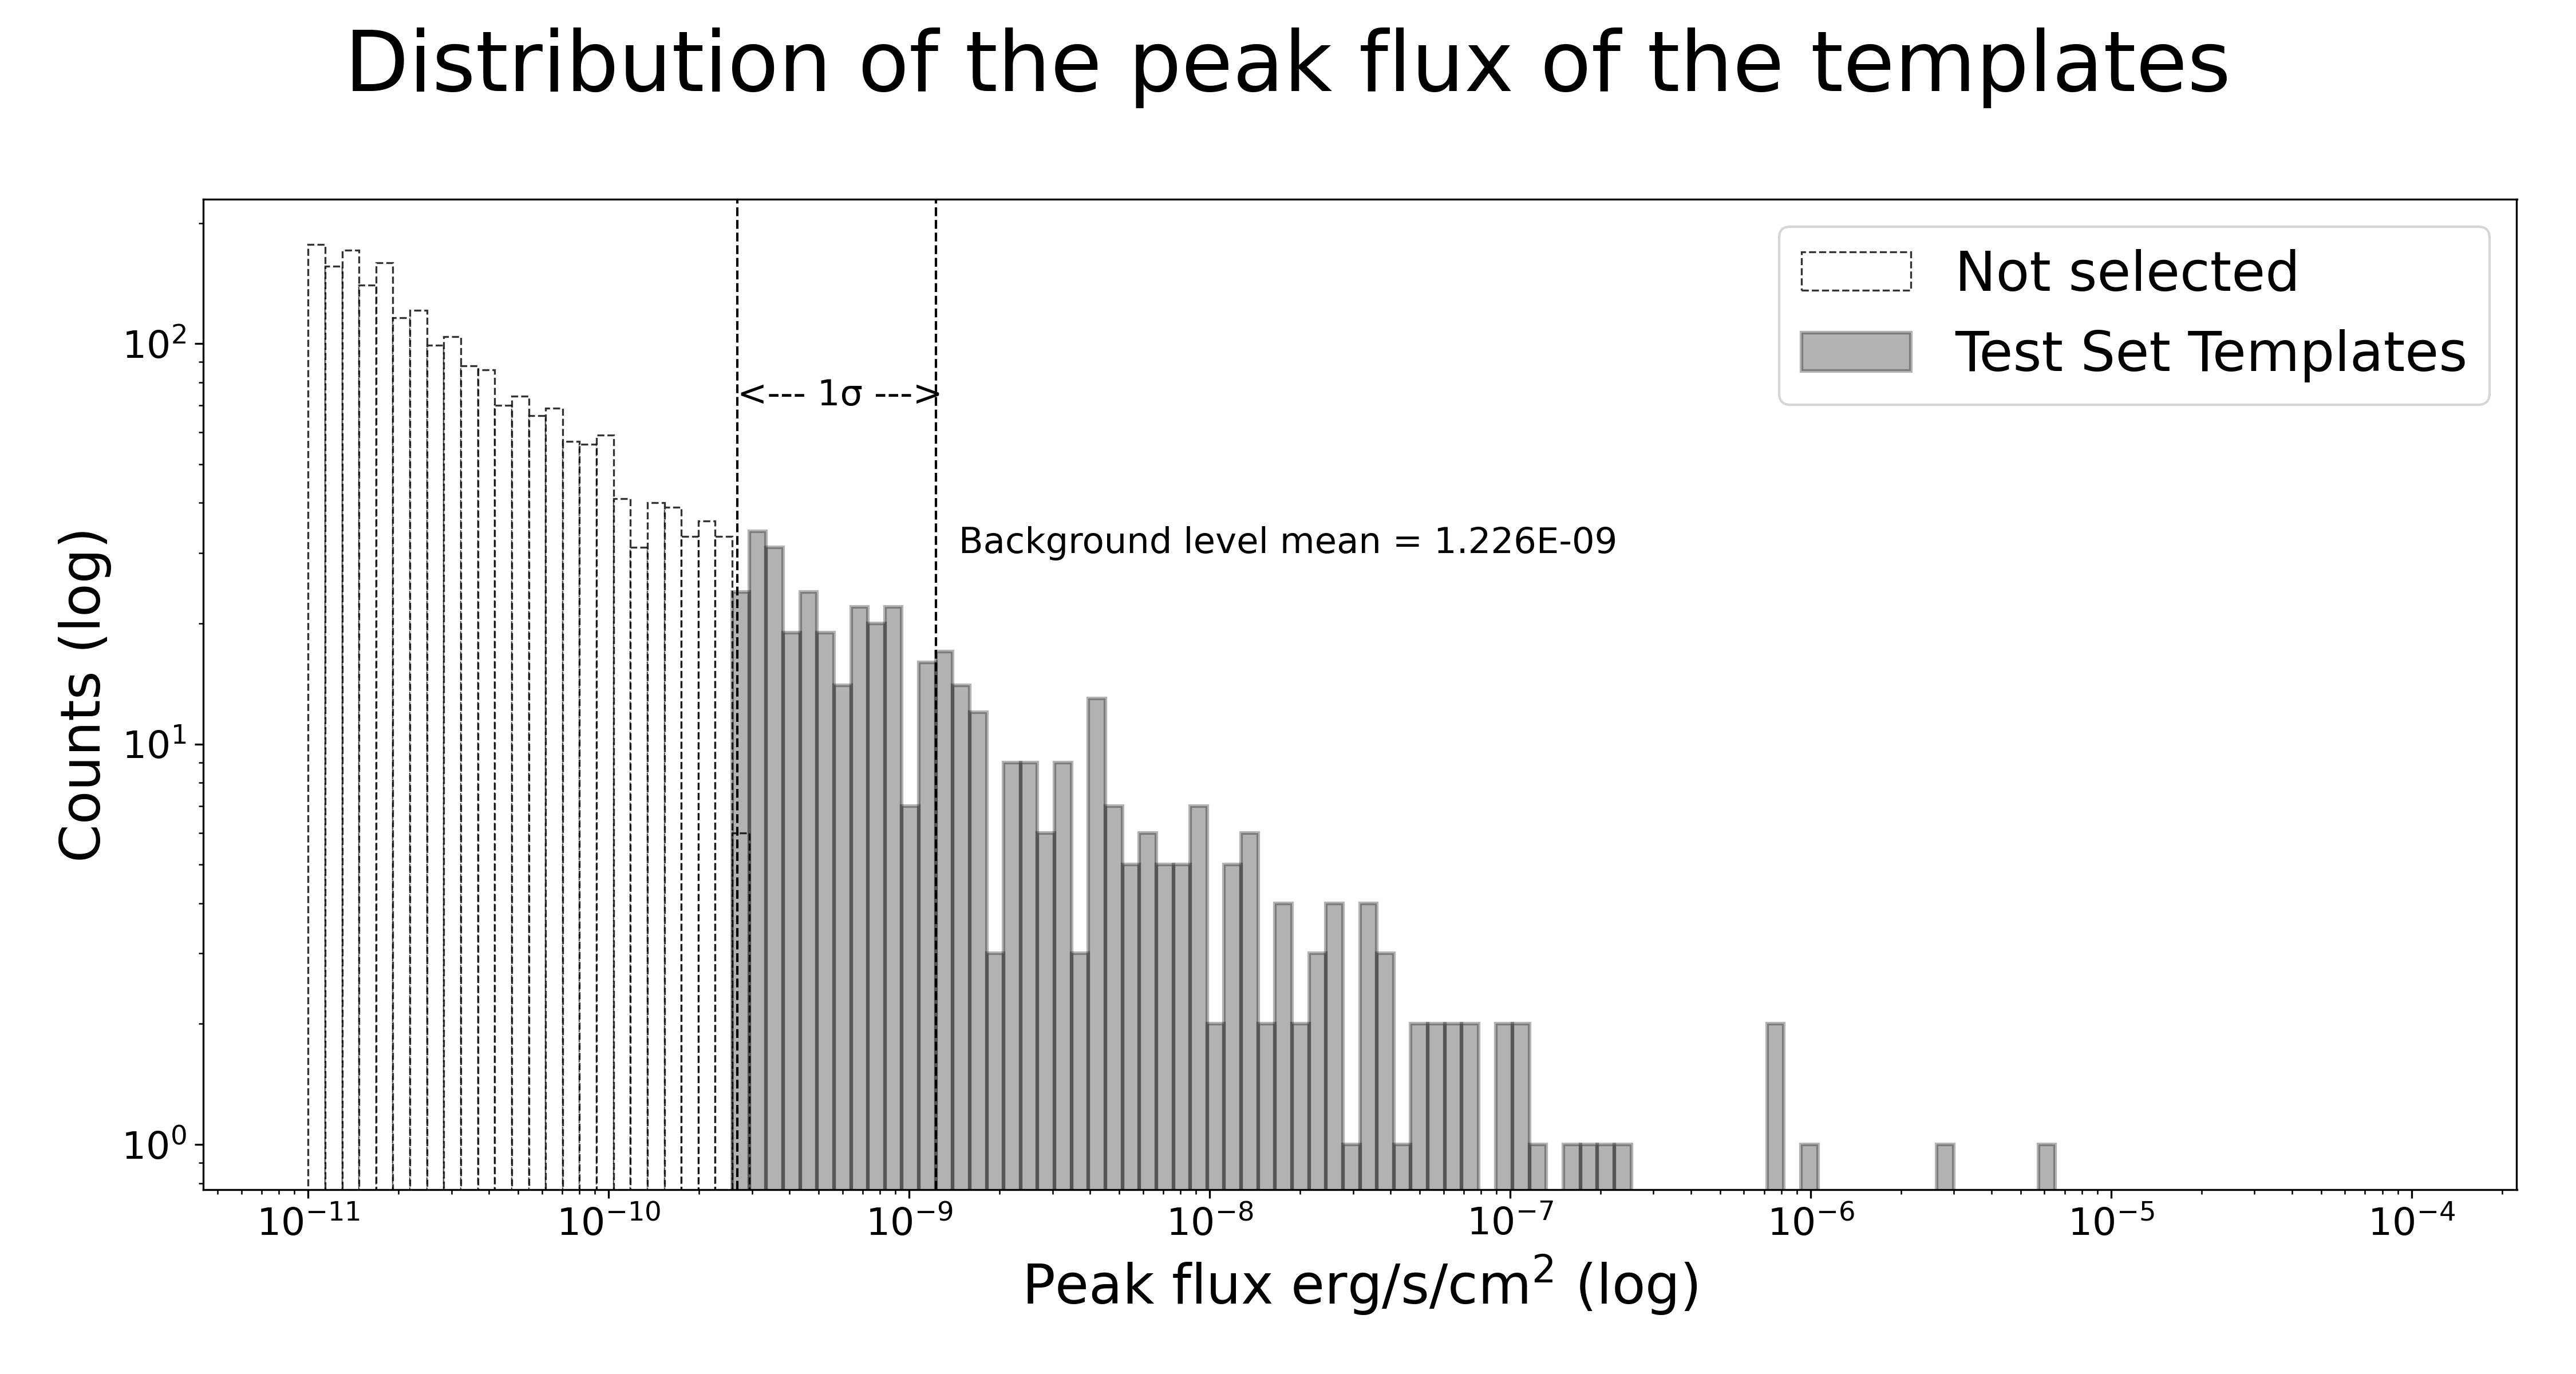
\includegraphics[width=1\textwidth]{figures/experiments/templates_max_flux_distributions.png}
\caption{The distribution of the peak flux for each GRB template. The selected templates are 419 and their peak fluxes are within the $[2.6785e-10, \infty]$ range.}
\label{f:exp-max-flux-distribution-E}
\end{figure}
The simulation time is limited to 500 seconds because we are interested in the first part of the GRB event, given the nature of the scientific use cases described in \autoref{s:contribution-2-use-cases}. The trigger time that defines the start of the GRB event is fixed and equal to 250 seconds. As described in \autoref{ss:integrator-module}, the photons lists must be integrated in space, time, and energy to generate the multi-variate time series of flux measurements. The integration time is set to 5 seconds to evaluate the performances of the techniques in the short-term scenario and 1 second for the very short-term scenario. The integration process generates time series of 100 (short-term scenario) and 500 (very short-term scenario) flux measurements. Finally, as described in \autoref{ss:extractor}, the time series extractor module extracts sub-sequences from the generated time series. The length of the sub-sequences is fixed and set to 5 points, the same setting used to generate the 
data to train the auto-encoder. The stride parameter is set to 1 because the A.D. technique can use overlapping temporal bins, drastically reducing the time the model waits for data during the online inference. In contrast, the Li\&Ma technique must use temporal bins that are statistically independent. Finally, since the test set must be supervised, each sub-sequence is associated with a label. A sub-sequence is labeled as anomalous if at least one of its points exceeds the trigger time threshold that defines the start of the GRB event. At the end of the data pipeline for the test set generation, in the short-term scenario (integration time equal to 5 seconds), the number of test samples is 40224, of which 20531 are labeled anomalous. In the very short-term scenario (integration time = 1 second), the number of test samples is 207824, of which 104331 are labeled anomalous.


\subsection{P-value thresholds}
\label{s:p-values-results}
The p-value analysis has been performed to compute the thresholds the models can use to issue detections (i.e., positive classification with a $5\sigma$ significance). The distributions of the reconstruction errors and the corresponding p-values for the A.D. technique with CNN and RNN implementations and for integration times equal to 5 and 1 seconds are shown in \autoref{s:appendix-pvalue}. \autoref{tab:p-val-thresholds-it-5} and \autoref{tab:p-val-thresholds-it-1} show the value of the thresholds that correspond to $5\sigma$ significance, for both RNN and CNN implementation and different integration times:
\begin{table}[ht]
\centering
\begin{tabular}{|c|c|c|}
    \hline
    Model & Threshold & Sigma \\ 
    \hline
    RNN & $0.0020$ & $5.048$ \\
    CNN & $0.0139$ & $5.046$ \\
    \hline
    \end{tabular}
\caption{The thresholds corresponding to $5\sigma$ classification in the short term scenario (integration time equals 5 seconds).}
\label{tab:p-val-thresholds-it-5}
\vspace{1cm}
\centering
\begin{tabular}{|c|c|c|}
    \hline
    Model & Threshold & Sigma \\ 
    \hline
    RNN & $0.0026$ & $5.041$ \\
    CNN & $0.0316$ & $5.048$ \\
    \hline
\end{tabular}
\caption{The thresholds corresponding to $5\sigma$ classification in the very short term scenario (integration time equals 1 second).}
\label{tab:p-val-thresholds-it-1}
\end{table}



 
\section{Results}
\label{s:Experiment-Results}

\subsection{Accuracy, precision, recall, and false positive rate}
\label{s:Acc-Fpr}
The accuracy, precision, recall, and false positive rate metrics tell us the percentage of the time series correctly classified, what proportion of positive identifications was actually correct, what proportion of actual positives was identified correctly, and what proportion of the actual negative events were wrongly categorized as positive. While precision measures the probability of a sample classified as positive to be an actual positive sample, the false positive rate measures the ratio of false positives within the negative samples. The accuracy, precision, and recall values for different thresholds can help understand the trade-off between the number of false positive and false negative classifications and also to compare the CNN and RNN implementations. The thresholds corresponding to $5\sigma$ significance have been used to evaluate these metrics. \autoref{s:appendix-metrics} shows the accuracy, precision, and recall curves for the A.D. technique with CNN and RNN implementation and for different integration times equal to 1 and 5 seconds. As we can see from \autoref{tab:standard-metrics}, the RNN performs better in terms of accuracy and recall in both scenarios. At the same time, CNN can optimize the number of false positive classifications. 

\begin{table}[ht]
\centering
\begin{tabular}{|c|c|c|c|c|}
    \hline
    Model & Accuracy & Precision & Recall & False Positive Rate \\ 
    \hline
    RNN & $61.81\%$ & $99.83\%$ & $25.22\%$ & $0.17\%$ \\
    CNN & $59.96\%$ & $99.86\%$ & $21.58\%$ & $0.13\%$ \\
    \hline
    \end{tabular}
\caption{Standard metrics in the short-term settings (integration time=5), using the $5\sigma$ threshold. The number of test samples is 40224, of which 20531 are anomalous.}
\vspace{1cm}
\centering
\begin{tabular}{|c|c|c|c|c|}
    \hline
    Model & Accuracy & Precision & Recall & False Positive Rate \\ 
    \hline
    RNN & $57.05\%$ & $99.97\%$ & $14.46\%$ & $0.033\%$ \\
    CNN & $55.58\%$ & $99.98\%$ & $11.52\%$ & $0.016\%$ \\
    \hline
\end{tabular}
\caption{Standard metrics in the very short-term settings (integration time=1), using the $5\sigma$ threshold. The number of test samples is 207824, of which 104331 are anomalous.}
\label{tab:standard-metrics}
\end{table}

\subsection{Serendipitous discoveries use case}
\label{s:Serendipitous-Discoveries-Results}
In the serendipitous discoveries scenario, a GRB event serendipitously appears in the telescopes' field of view. The goal is to detect the event to broadcast a science alert. The detection must be performed as soon as possible for two main reasons: the GRB events are transient, and the first seconds of data provide crucial information about the initial conditions of the GRB, such as the properties of the central engine and the nature of the emitting material \cite{kumar2000energetics}.

\subsubsection{Short-term scenario (integration time equals to 5 seconds)}
\label{s:Serendipitous-Discoveries-Results-Short-Term}
\autoref{f:cumulative-detections-itime-5} shows the cumulative number of detections done by the A.D. and Li\&Ma techniques for each temporal bin in the short-term scenario. The x-axis holds each temporal bin. The y-axis holds the cumulative number of detections among all the simulated trials.
\begin{figure}[ht]
\centering
\includesvg[width=1\textwidth]{figures/experiments/results/ad_vs_li_cumulative_test_set_all_itime_5.svg}
\caption{The cumulative number of detections among all simulated trials for each time bin in the short-term scenario (integration time equal to 5 seconds) for the A.D. (CNN and RNN implementations) and Li\&Ma techniques. The vertical dashed line corresponds to the start of the GRB event.}
\label{f:cumulative-detections-itime-5}
\end{figure}
The plot shows the robustness of the Li\&Ma technique, detecting more GRBs than the A.D. technique. It also shows that the Li\&Ma technique can be applied only for temporal bins that do not overlap, i.e., statistically independent. In contrast, the A.D. technique can be applied to each $T=5$ seconds of new data, leading to faster detections. This feature is essential since the detections must be performed as soon as possible. To give a quantitative measure of the quickness to perform detections, a metric called \textit{detection delay} has been defined as the average time of the first detection for each GRB event.
\begin{table}[ht] %%%%%%%%%%%%%%%%%%%%%%%%%%%%%%%%%%%%%%%%%%%%%%%%%%%%%%%%%%%%%% detections it=5
\centering
\begin{tabular}{|c|cccc|} 
\hline
\multicolumn{1}{|c|}{A.D. vs Li\&Ma} & \multicolumn{4}{c|}{$T_{max}$}  \\
    & $TT+15s$ & $TT+30s$ &  $TT+60s$ & $TT+120s$  \\
\hline
Number of detections (RNN) & 45 & 90 & 116  & 132 \\
\hline
Number of detections (CNN) & 40 & 65 & 99 & 118 \\
\hline
Number of detections (Li\&Ma) & 0 & 82 & 137 & 167 \\
\hline
Detection delay (s) (RNN) & $11.11 \pm 3.78$ & $18.17 \pm 8.08$  & $24.74 \pm 14.71$   & $32.01 \pm 24.41$ \\
\hline
Detection delay (s) (CNN)& $11.62 \pm 3.6$ & $16.69 \pm 7.35$ & $26.41 \pm 15.46$  & $36.02 \pm 26.91$ \\
\hline
Detection delay (s) (Li\&Ma)& - & $25 \pm 0$ & $35.04 \pm 12.25$  & $43.86 \pm 22.47$ \\
\hline
\end{tabular}
\caption{The table reports the number of serendipitous detections in the short-term scenario (integration time equal to 5 seconds) starting from the beginning of the GRB event ($TT=250s$) within a $T_{max}$ time and the corresponding detection delay. The detection delay is the average time the techniques take to detect the GRB events for the first time.}
\label{tab:serendipitous-detections-itime-5}
\end{table}
\begin{table}[ht] %%%%%%%%%%%%%%%%%%%%%%%%%%%%%%%%%%%%%%%%%%%%%%%%%%%%%%%%%%%%%% detections it=1
\centering
\begin{tabular}{|c|cccc|} 
\hline
\multicolumn{1}{|c|}{A.D. vs Li\&Ma} & \multicolumn{4}{c|}{$T_{max}$}  \\
    & $TT+15s$ & $TT+30s$ &  $TT+60s$ & $TT+120s$  \\
\hline
Number of detections (RNN) & 42 & 70 & 92  & 110 \\
\hline
Number of detections (CNN) & 38 & 59 & 74 & 79 \\
\hline
Number of detections (Li\&Ma) & 24 & 50 & 84 & 97 \\
\hline
Detection delay (s) (RNN) & $8.12 \pm 4.18$ & $13.6 \pm 7.91$  & $20.54 \pm 14.7$   & $31.65 \pm 29.36$ \\
\hline
Detection delay (s) (CNN)& $8.66 \pm 4.07$ & $14.25 \pm 8.62$ & $19.24 \pm 12.82$  & $22.42 \pm 17.56$ \\
\hline
Detection delay (s) (Li\&Ma)& $11.46 \pm 3.67$ & $18.1 \pm 7.54$ & $29.46 \pm 16.04$  & $36.91 \pm 24.71$ \\
\hline
\end{tabular}
\caption{The table reports the number of serendipitous detections in the very short-term scenario (integration time equal to 1 second) starting from the beginning of the GRB event ($TT=250s$) within a $T_{max}$ time and the corresponding detection delay. The detection delay is the average time the techniques take to detect the GRB events for the first time.}
\label{tab:serendipitous-detections-itime-1}
\end{table}
\begin{table}[ht] %%%%%%%%%%%%%%%%%%%%%%%%%%%%%%%%%%%%%%%%%%%%%%%%%%%%%%%%%%%%%% common detections it=5
\begin{tabular}{|c|cccc|}  
\hline
\multicolumn{1}{|c|}{A.D. (RNN) vs Li\&Ma} & \multicolumn{4}{c|}{$T_{max}$}  \\
(common detections) & $TT+15s$ & $TT+30s$ &  $TT+60s$ & $TT+120s$        \\
\hline
Number of detections & 0 & 69 & 109 & 129           \\
\hline
Detection delay (s) (RNN)& - & $15.87 \pm 6.7$ & $24.08 \pm 13.72 $ & $32.56 \pm 24.42.2$        \\
\hline
Detection delay (s) (Li\&Ma)& - & $25 \pm 0$ & $34.17 \pm 12.05$  & $39.53 \pm 17.8$   \\
\hline
\end{tabular}
\vspace{1em}
\begin{tabular}{|c|cccc|}
\hline
\multicolumn{1}{|c|}{A.D. (CNN) vs Li\&Ma} & \multicolumn{4}{c|}{$T_{max}$}  \\
(common detections) & $TT+15s$ & $TT+30s$ &  $TT+60s$ & $TT+120s$        \\
\hline
Number of detections & 0 & 61 & 96 & 116           \\
\hline
Detection delay (s) (CNN)& - & $16.15 \pm 7.09$ & $26.2 \pm 15.27$  & $36.29 \pm 27.05$         \\
\hline
Detection delay (s) (Li\&Ma)& - & $25 \pm 0$ & $34.17 \pm 12.05$  & $39.53 \pm 17.8$   \\
\hline
\end{tabular}
\caption{The tables report the number of serendipitous common detections in the short-term scenario (integration time equal to 5 seconds) starting from the beginning of the GRB event ($TT=250s$) within a $T_{max}$ time and the corresponding detection delay. The detection delay is the average time the techniques take to detect the GRB events for the first time.}
\label{tab:serendipitous-detections-common-itime-5}
\end{table}
\begin{table} %%%%%%%%%%%%%%%%%%%%%%%%%%%%%%%%%%%%%%%%%%%%%%%%%%%%%%%%%%%%%%  common detections it=1
\begin{tabular}{|c|cccc|}  
\hline
\multicolumn{1}{|c|}{A.D. (RNN) vs Li\&Ma} & \multicolumn{4}{c|}{$T_{max}$}  \\
(common detections) & $TT+15s$ & $TT+30s$ &  $TT+60s$ & $TT+120s$        \\
\hline
Number of detections & 23 & 45 & 80 & 94 \\
\hline
Detection delay (s) (RNN)& $8.22 \pm 4.02$ & $14.44 \pm 8.08 $ & $21.24 \pm 14.29$ & $ 27.1 \pm 22.92$ \\
\hline
Detection delay (s) (Li\&Ma)& $11.74 \pm 3.49$ & $17.33 \pm 6.8$ & $29.12 \pm 15.83$  & $36.38 \pm 23.83$   \\
\hline
\end{tabular}
\vspace{1em}
\begin{tabular}{|c|cccc|}
\hline
\multicolumn{1}{|c|}{A.D. (CNN) vs Li\&Ma} & \multicolumn{4}{c|}{$T_{max}$}  \\
(common detections) & $TT+15s$ & $TT+30s$ &  $TT+60s$ & $TT+120s$        \\
\hline
Number of detections & 21 & 38 & 64 & 74           \\
\hline
Detection delay (s) (CNN) & $7.81 \pm 4.03$ & $14.18 \pm 8.83$  & $19.58 \pm 12.62$  & $23.51 \pm 17.58$  \\
\hline
Detection delay (s) (Li\&Ma)& $11.43 \pm 3.5$ & $16.45 \pm 6.78$ & $25.7 \pm 14.47$  & $30.27 \pm 19.61$   \\
\hline
\end{tabular}
\caption{The tables report the number of serendipitous common detections in the very short-term scenario (integration time equal to 1 second) starting from the beginning of the GRB event ($TT=250s$) within a $T_{max}$ time and the corresponding detection delay. The detection delay is the average time the techniques take to detect the GRB events for the first time.}
\label{tab:serendipitous-detections-common-itime-1}
\end{table}
\autoref{tab:serendipitous-detections-itime-5} shows the performances of the A.D. (RNN and CNN implementations) and Li\&Ma techniques in terms of the number of detections starting from the beginning of the GRB event ($TT = 250s$)  within a $T_{max}$ time. $T_{max}$ represents the delay before the start of the observation when the observatory reacts to an external science alert, assuming the following values: 15, 30, 60, and 120 seconds. The tables also report the detection delays. In \autoref{tab:serendipitous-detections-common-itime-5}, only the common GRB detections between A.D. and Li\&Ma have been considered to give a more accurate comparison of the detection delay. Both tables show lower detection delays for the A.D. technique, regardless of the layer's implementations. This result demonstrates that the anomaly detection technique is more suitable in situations where the detection time needs to be optimized.
% seen / not seen
\begin{table}[ht] %%%%%%%%%%%%%%%%%%%%%%%%%%%%%%%%%%%%%%%%%%%%%%% seen-not-seen it=5
\centering
\begin{tabular}{|r|c|c|c|}
\hline
\multicolumn{1}{|c|}{\diagbox{Detected by}{Not detected by}} & A.D. (RNN) & A.D. (CNN) & LiMa  \\
\hline
A.D. (RNN) & -          & 1          & 3     \\
\hline
A.D. (CNN) & 0          & -          & 1 \\
\hline
Li\&Ma     & 0         & 0         & -    \\
\hline
\end{tabular}
\begin{tabular}{|r|c|c|c|}
\hline
\multicolumn{1}{|c|}{\diagbox{Detected by}{Not detected by}} & A.D. (RNN) & A.D. (CNN) & LiMa  \\
\hline
A.D. (RNN) & -          & 2          & 3     \\
\hline
A.D. (CNN) & 0          & -          & 2     \\
\hline
Li\&Ma & 11         & 13         & -    \\
\hline
\end{tabular}
\begin{tabular}{|r|c|c|c|}
\hline
\multicolumn{1}{|c|}{\diagbox{Detected by}{Not detected by}} & A.D. (RNN) & A.D. (CNN) & LiMa  \\
\hline
A.D. (RNN) & -          & 3         & 3     \\
\hline
A.D. (CNN) & 0          & -          & 2     \\
\hline
Li\&Ma & 18         & 25         & -    \\
\hline
\end{tabular}
\begin{tabular}{|r|c|c|c|}
\hline
\multicolumn{1}{|c|}{\diagbox{Detected by}{Not detected by}} & A.D. (RNN) & A.D. (CNN) & LiMa  \\
\hline
A.D. (RNN) & -          & 5          & 3     \\
\hline
A.D. (CNN) & 0          & -          & 2     \\
\hline
Li\&Ma & 28         & 39         & -    \\
\hline
\end{tabular}
\caption{The number of GRB events serendipitous detected in the short-term scenario (integration time equal to 5 seconds) by a technique but not detected by the others, within $T_{max}=TT+15$, $T_{max}=TT+30$, $T_{max}=TT+60$, and $T_{max}=TT+120$ seconds.}
\label{tab:seen-unseen-serendipitous-itime-5}
\end{table}
In the same settings, we are also interested in the number of GRB events detected by the A.D. technique but not detected by the Li\&Ma technique: \autoref{tab:seen-unseen-serendipitous-itime-5} is a confusion matrix showing that the A.D. technique with RNN layers found 3 GRB events and the A.D. with CNN layers found 2. 

\subsection{Serendipitous discoveries use case in the very short-term scenario}
\label{s:Serendipitous-Discoveries-Results-very-short-term}
The evaluations of the previous section will be performed again in the very short-term scenario, where the integration time equals 1 second. In this scenario, the photons counts are further reduced, often exceeding the lower bounds of the Li\&Ma technique (equal to 10). Hence, this technique is not always applicable. The reduced number of photon counts also negatively affects the performance of the A.D. technique. In contrast, it further reduces the time the A.D. technique needs to wait for new data: from 5 seconds to 1 second. Each second, a new flux data measurement is available, and a new sub-sequence is ready for analysis. This potentially decreases the detection time, leading to better performance. \autoref{f:cumulative-detections-itime-1} shows the cumulative number of detections done by the A.D. and Li\&Ma techniques for each temporal bin in the very short-term scenario. The x-axis holds each temporal bin. The y-axis holds the cumulative number of detections among all the simulated trials. The number of detections performed by the A.D. technique with RNN implementation is always greater than the number of detections performed by the Li\&Ma technique, proving greater robustness in this extreme scenario. The Li\&Ma technique suffers from its limitation of having at least 10 photon counts of applying the analysis. In contrast, the A.D. method overcomes this limitation and still performs detections. Also, in the very short-term scenario, \autoref{tab:serendipitous-detections-itime-1} and \autoref{tab:serendipitous-detections-common-itime-5} show that the A.D. technique performs faster detections, obtaining a detection delay always lower than the Li\&Ma technique. \autoref{tab:seen-unseen-serendipitous-itime-1} shows that the A.D. technique detects from 5 to 11 GRB events not seen by the Li\&Ma technique, but in this case, this is not very interesting since the A.D technique sees the majority of the GRB events. These results also confirm that the RNN implementation performs better than the CNN implementation. 
\begin{figure}[ht] %%%%%%%%%%%%%%%%%%%%%%%%%%%%%%%%%%%%%%%%%%%%%%%%%%%%%%%%%%%%%%%%%
\centering
\includesvg[width=1\textwidth]{figures/experiments/results/ad_vs_li_cumulative_test_set_all_itime_1.svg}
\caption{The cumulative number of detections among all simulated trials for each time bin in the very short-term scenario (integration time equal to 1 second) for the A.D. (CNN and RNN implementations) and Li\&Ma techniques. The vertical dashed line corresponds to the start of the GRB event.}
\label{f:cumulative-detections-itime-1}
\end{figure}
\begin{table} %%%%%%%%%%%%%%%%%%%%%%%%%%%%%%%%%%%%%%%%%%%%%%%%%%%%%%%%%%%%%% seen not seen it=1
\centering
\begin{tabular}{|r|c|c|c|}
\hline
\multicolumn{1}{|c|}{\diagbox{Detected by}{Not detected by}} & A.D. (RNN) & A.D. (CNN) & LiMa  \\
\hline
A.D. (RNN) & -          & 1          & 6     \\
\hline
A.D. (CNN) & 0          & -          & 5 \\
\hline
Li\&Ma     & 1         & 1         & -    \\
\hline
\end{tabular}
\begin{tabular}{|r|c|c|c|}
\hline
\multicolumn{1}{|c|}{\diagbox{Detected by}{Not detected by}} & A.D. (RNN) & A.D. (CNN) & LiMa  \\
\hline
A.D. (RNN) & -          & 4          & 6     \\
\hline
A.D. (CNN) & 0          & -          & 5     \\
\hline
Li\&Ma & 1         & 3         & -    \\
\hline
\end{tabular}
\begin{tabular}{|r|c|c|c|} 
\hline
\multicolumn{1}{|c|}{\diagbox{Detected by}{Not detected by}} & A.D. (RNN) & A.D. (CNN) & LiMa  \\
\hline
A.D. (RNN) & -          & 9         & 6     \\
\hline
A.D. (CNN) & 0          & -          & 5     \\
\hline
Li\&Ma & 1         & 10         & -    \\
\hline
\end{tabular}
\begin{tabular}{|r|c|c|c|}
\hline
\multicolumn{1}{|c|}{\diagbox{Detected by}{Not detected by}} & A.D. (RNN) & A.D. (CNN) & LiMa  \\
\hline
A.D. (RNN) & -          & 20          & 11    \\
\hline
A.D. (CNN) & 0          & -          & 5     \\
\hline
Li\&Ma & 2         & 14         & -    \\
\hline
\end{tabular}
\caption{The number of GRB events serendipitous detected in the very short-term scenario (integration time equal to 1 second) by a technique but not detected by the others, within $T_{max}=TT+15$, $T_{max}=TT+30$, $T_{max}=TT+60$, and $T_{max}=TT+120$ seconds.}
\label{tab:seen-unseen-serendipitous-itime-1}
\end{table}

\subsubsection{Short-term vs very short-term for serendipitous discoveries}
\label{s:serendipitous-short-term-vs-very-short-term}
The previous sections show the superiority of the A.D. technique concerning Li\&Ma. In this section, we want to understand the best scenario for applying the A.D. technique for serendipitous discoveries. Let's compare the results in \autoref{tab:serendipitous-detections-itime-5} and \autoref{tab:serendipitous-detections-itime-1}. If the goal is to maximize the number of detections, the short-term scenario with an integration time of 5 seconds is preferred. If the goal is to optimize the detection delay, the very short-term scenario with an integration time of 1 second is the way to go. In practice, the two scenarios are not exclusive, and both models can work together in parallel. 


\subsection{Observation triggered by an external science alert use case}
\label{s:Science-Alert-Results}

When the observatory reacts to a science alert another facility broadcasts, the telescopes will change their pointing to observe a sky region where a GRB event is already started. The time taken to receive the science alert, change the pointing, and wait for enough data to perform the first analysis is variable: four values have been considered to model this delay: 15, 30, 60, and 120 seconds. The same evaluation done for the serendipitous discovery use case is performed in this section. The only difference is that the observation starts at time $TT+120$ until the end of the observation (500 seconds).

\begin{figure}[ht] %%%%%%%%%%%%%%%%%%%%%%%%%%%%%%%%%%%% cumulative it=5
\centering
\includesvg[width=1\textwidth]{figures/experiments/results/ad_vs_li_cumulative_test_set_all_itime_5_45_95.svg}
\caption{The cumulative number of detections among all simulated trials for each time bin in the short-term scenario (integration time equal to 5 seconds) for the A.D. (CNN and RNN implementations) and Li\&Ma techniques. The vertical dashed line corresponds to the start of the GRB event.}
\label{f:cumulative-detections-science-alert-itime-5}
\end{figure}

\begin{figure}[ht] %%%%%%%%%%%%%%%%%%%%%%%%%%%%%%%%%%%%%%%% cumulative it=1
\centering
\includesvg[width=1\textwidth]{figures/experiments/results/ad_vs_li_cumulative_test_set_all_itime_1_240_500.svg}
\caption{The cumulative number of detections among all simulated trials for each time bin in the very short-term scenario (integration time equal to 1 second) for the A.D. (CNN and RNN implementations) and Li\&Ma techniques. The vertical dashed line corresponds to the start of the GRB event.}
\label{f:cumulative-detections-science-alert--itime-5}
\end{figure}







\section{Summary}
\label{s:Experiments-Summary}
